\documentclass[14pt]{mmcs_article}
\usepackage[russian]{babel}
\usepackage{url}
\usepackage{amsmath, amsthm, amsfonts, amssymb}
\graphicspath{{images/}}%путь к рисункам
\usepackage{svg}  % опция clean удаляет временные файлы
\setsvg{inkscapelatex=true} % глобальная настройка для обработки текста
\svgpath{images/}%путь к рисункам
\usepackage{multirow}
\usepackage{enumitem} 
\begin{document}
	
	% Титульные листы
	% раскомментировать требуемое
	%\include{Titul3k} % для курсовой
	\include{TitulBak}% для работы бакалавра
	%\include{TitulMag}% для работы магистра
	
	\renewcommand{\contentsname}{Оглавление}
	
	\tableofcontents
	
	%=======================
	\newpage
	\section{Введение}
	Рассмотренная в предыдущем аналитическом отчете «Разработка байесовской статистической модели для определения
	ширины окна аномалии парадоксального сна животного,
	вызванной предвестниками крупного сейсмического события,
	на основе биоэлектрического сигнала мозга» байесовская
	changepoint-модель была реализована с помощью библиотеки PyMC. Cхема модели представленна на рисунке \ref{fig:grafviz}. Код модели представлен на листинге \ref{app-lst:bayes-model}.
	
		\begin{figure}[H]
		\includesvg[width=\textwidth, inkscapelatex=false]{grafviz.svg}
		\caption{Схема модели поиска точки разладки.}
		\label{fig:grafviz} % Метка для ссылки
	\end{figure}
	
	\section{Полный перебор по метрике LOO-ELPD}
	
	\subsection*{Постановка задачи выбора модели}
	 Такая байесовская
	 changepoint-модель представляет собой не единичную модель, а
	семейство моделей, порождаемое комбинациями факторов
	предобработки данных и статистических спецификаций. Каждая
	комбинация определяет отдельную вероятностную модель,
	характеризующуюся собственными предсказаниями о положении
	точки разладки $\tau$ и величине параметрического сдвига.
	В связи с этим возникает задача определения конфигурации,
	наилучшим образом описывающей наблюдаемые данные.
	
	Поскольку цель работы состоит не в подгонке параметров под
	имеющуюся выборку, а в проверке устойчивости выявленных
	закономерностей, сравнение моделей проводится по их
	\textbf{предсказательной способности} — качеству прогноза
	на новых наблюдениях, не использовавшихся при обучении.
	
	\subsection*{Пространство перебора}
	
	Факторы, определяющие конкретную конфигурацию модели, можно
	разделить на две группы: параметры предобработки временных
	рядов и параметры вероятностной модели.
	
	\textbf{Параметры предобработки:}
	\begin{itemize}
		\item \textbf{Ширина скользящего окна} $W \in \{2, 3, 6\}$~ч. —
		определяет, за какой временной интервал вычисляется доля
		парадоксального сна (REM\%).
		\item \textbf{Шаг смещения окна} $S \in \{1, 2\}$~ч. — 
		задает частоту, с которой вычисляются значения REM\%.
		\item \textbf{Группировка чанков}
		$\in \{\text{concat}, \text{odd}, \text{even}\}$. —
		способ объединения чанков для вычисления описательных
		статистик: \texttt{concat} объединяет четный и соседний
		нечетный чанк (16 чанков $\to$ 8 пар) для получения
		суточной метрики; \texttt{odd} использует только
		нечетные чанки (условно «дневные»); \texttt{even} —
		только четные (условно «ночные»). Во всех случаях
		результатом является ряд длиной 8 значений на признак.
		\item \textbf{Набор статистик чанков}
		$\subseteq \{\text{mean}, \text{range}\}$. —
		описательные статистики, вычисляемые внутри каждого чанка
		(или пары чанков для \texttt{concat}): среднее и размах.
	\end{itemize}
	
	\textbf{Параметры вероятностной модели:}
	\begin{itemize}
		\item \textbf{Семейство правдоподобия}
		$\in \{\text{student\_t}, \text{lognormal}, \text{beta}\}$. —
		распределение, которым описывается каждый признак в фоновом
		и аномальном режимах. Выбор конкретных семейств для каждого
		признака обусловлен априорными представлениями о природе
		соответствующих статистик. Так, для признака \texttt{mean}
		(средняя доля REM) допустимыми являются \texttt{student\_t}
		и \texttt{lognormal}, поскольку среднее нормированного
		профиля принимает значения на положительной полуоси и может
		иметь тяжелые хвосты. Для признака \texttt{range} (размах)
		рассматриваются \texttt{lognormal} и \texttt{beta}, так как
		размах ограничен интервалом $[0, 1]$ после минимаксной
		нормировки, а \texttt{beta}-распределение является
		естественной моделью для величин на единичном отрезке.
	\end{itemize}
	
	Полное декартово произведение перечисленных факторов образует
	конечное, но достаточно обширное пространство конфигураций.
	Стратегия \textbf{полного перебора} (exhaustive search)
	заключается в том, чтобы построить, обучить (провести
	MCMC-сэмплирование) и оценить качество \textit{каждой}
	конфигурации из этого пространства. Такой подход, в отличие от
	жадных или эволюционных стратегий поиска, гарантирует, что мы
	не пропустим локально оптимальное решение и получим полную
	картину того, как различные факторы влияют на предсказательную
	силу модели.
	
	\subsection*{Кросс-валидация временных рядов по методу LOO}
	
	Традиционная перекрестная проверка (cross--validation)
	оценивает\linebreak обобщающую способность модели, разбивая данные на
	обучающую и проверочную части, обучая модель на первой и
	измеряя ошибку предсказаний на второй. В случае независимых
	наблюдений стандартным подходом является $k$-кратная
	кросс-валидация со случайным разбиением на блоки. Однако для
	временных рядов такой подход неприменим: случайное
	перемешивание разрушает временную структуру и создает
	нереалистично оптимистичные оценки, поскольку модель получает
	доступ к <<будущим>> наблюдениям \cite{Bergmeir2012}.
	
	Альтернативой служит \textbf{leave-one-out кросс-валидация}
	(LOO-CV), адаптированная для временных рядов. В этом методе из
	обучающей выборки последовательно исключается ровно одно
	наблюдение (в нашем случае — одно сейсмическое событие),
	модель переобучается на оставшихся $E-1$ событиях, после чего
	вычисляется логарифмическое правдоподобие исключенного события
	при найденных параметрах. Процедура повторяется для каждого
	события, давая вектор из $E$ значений логарифмического
	правдоподобия.
	
	\subsection*{LOO-ELPD и преимущество перед наивным LOO}
	
	Наивная LOO-оценка ожидаемой логарифмической предсказательной
	плотности (expected log predictive density, ELPD) определяется
	как сумма логарифмических правдоподобий на отложенных
	наблюдениях \cite{Vehtari2017}:
	\begin{equation}\label{eq:naive_elpd}
		\widehat{\mathrm{elpd}}_{\mathrm{LOO}} = 
		\sum_{e=1}^{E} \log p(\mathcal{D}_e \mid \mathcal{D}_{-e}),
	\end{equation}
	где $\mathcal{D}_e$ — данные $e$-го сейсмического события,
	$\mathcal{D}_{-e}$ — все события, кроме $e$-го, а
	$p(\mathcal{D}_e \mid \mathcal{D}_{-e})$ — предсказательная
	плотность для $e$-го события, полученная путем усреднения
	правдоподобия по апостериорным параметрам, найденным по
	$\mathcal{D}_{-e}$.
	
	Основная проблема формулы \eqref{eq:naive_elpd} в том, что она
	требует \textit{полного переобучения} модели $E$ раз, по
	одному разу для каждого исключаемого события
	\cite{Vehtari2017}. При байесовском MCMC-сэмплировании, где
	обучение одной модели может занимать минуты или десятки минут,
	такая процедура становится вычислительно непозволительной для
	пространства из сотен или тысяч конфигураций.
	
	Решением служит \textbf{приближение Парето-сглаженной важности
		выборки} (Pareto-smoothed importance sampling, PSIS),
	предложенное в работе \cite{Vehtari2017} и реализованное в
	библиотеке ArviZ \cite{Kumar2019}. Ключевая идея метода состоит
	в том, чтобы обучить модель \textit{единожды} на всех $E$
	событиях, а затем оценить вклад каждого наблюдения в
	апостериорное распределение с помощью перевзвешивания
	важностных весов. Иными словами, вместо того чтобы исключать
	событие и переучиваться, мы корректируем вклад этого события в
	уже вычисленное полное апостериорное распределение.
	
	Формально, пусть $\boldsymbol{\theta}^{(s)} \sim
	p(\boldsymbol{\theta} \mid \mathcal{D})$ для $s = 1, \dots, S$ —
	выборочные значения параметров из полного апостериорного
	распределения. Стабилизированные важностные веса $w_e^{(s)}$
	для события $e$ определяются через отношение правдоподобий с
	последующим сглаживанием хвостов распределения весов с помощью
	аппроксимации обобщенным распределением Парето. Тогда
	PSIS-оценка ELPD принимает вид:
	\begin{equation}\label{eq:psis_elpd}
		\widehat{\mathrm{elpd}}_{\mathrm{LOO}} = 
		\sum_{e=1}^{E} \log \left( 
		\frac{ \sum_{s=1}^{S} w_e^{(s)} \, 
			p(\mathcal{D}_e \mid \boldsymbol{\theta}^{(s)}) }
		{ \sum_{s=1}^{S} w_e^{(s)} }
		\right).
	\end{equation}
	
	Данная оценка асимптотически эквивалентна наивной LOO-CV, но
	требует лишь одного запуска MCMC, а не $E$ запусков
	\cite{Vehtari2017}. Вычислительная экономия достигает
	$E$-кратного размера, что и делает полный перебор практически
	осуществимым в рамках данной работы.
	
	\subsection*{Особенности вычисления ELPD для многомерных событий}
	
	В стандартной постановке PSIS-LOO каждое <<наблюдение>> $y_i$
	представляет собой отдельное измерение — скалярную величину.
	Однако в нашей задаче одно наблюдение — это \textbf{целое
		сейсмическое событие}, описываемое многомерным временным рядом
	признаков парадоксального сна. Каждое событие $e$
	характеризуется набором из $F$ активных признаков (например,
	среднее и размах профиля REM), каждый из которых представлен
	вектором из $T$ временных чанков (отсчетов) ($T = 8$ для всех типов
	группировки: \texttt{even}, \texttt{odd} и \texttt{concat}).
	Таким образом, полная размерность одного события составляет
	$M = F \times T$ скалярных измерений.
	
	Предполагая условную независимость признаков при
	фиксированных параметрах модели, совместное правдоподобие
	события $e$ факторизуется в произведение правдоподобий
	отдельных измерений:
	\begin{equation}
		p(\mathcal{D}_e \mid \boldsymbol{\theta}) = 
		\prod_{f=1}^{F} \prod_{t=1}^{T} 
		p(y_{e,f,t} \mid \boldsymbol{\theta}_f),
	\end{equation}
	где $\boldsymbol{\theta}_f$ — параметры распределения для
	$f$-го признака. Соответственно, логарифмическое
	правдоподобие события есть сумма логарифмов:
	\begin{equation}
		\log p(\mathcal{D}_e \mid \boldsymbol{\theta}) = 
		\sum_{f=1}^{F} \sum_{t=1}^{T} 
		\log p(y_{e,f,t} \mid \boldsymbol{\theta}_f).
	\end{equation}
	
	Из этого следует, что вклад каждого события в итоговый
	$\widehat{\mathrm{elpd}}_{\mathrm{LOO}}$ пропорционален числу
	активных признаков $F$. Модель, использующая 5 признаков, будет
	иметь суммарный ELPD примерно в 5 раз больший, чем модель с
	одним признаком, даже если дополнительные признаки не несут
	содержательной информации о предсейсмических изменениях. По этой
	причине прямое сравнение моделей с разным числом признаков по
	суммарному ELPD некорректно.
	
	Для обеспечения сопоставимости моделей вводится
	\textbf{нормированный} показатель — ожидаемая логарифмическая
	предсказательная плотность \textbf{в расчете на один признак}:
	\begin{equation}\label{eq:elpd_per_feature}
		\overline{\mathrm{elpd}}_{\mathrm{LOO}} = 
		\frac{\widehat{\mathrm{elpd}}_{\mathrm{LOO}}}{F},
	\end{equation}
	где $F$ — число активных признаков в данной конфигурации.
	
	%Нормировка на число событий $E$ не требуется в основном
	%переборе, поскольку все модели оцениваются на одной и той же
	%выборке, и $E$ является константой для всех конфигураций.
	%Однако, как будет показано ниже, при исключении влиятельных
	%событий разными моделями число событий может различаться, и в
	%этом случае необходима дополнительная нормировка.
	
	\subsection*{Диагностика Парето $\hat{k}$}
	
	Качество PSIS-приближения контролируется с помощью
	диагностики \textbf{Парето $\hat{k}$}. Для каждого наблюдения
	$e$ вычисляется оценка параметра формы обобщенного
	распределения Парето $\hat{k}_e$, которая характеризует
	толщину хвоста распределения важностных весов
	\cite{Vehtari2017, Vehtari2024}:
	
	\begin{itemize}
		\item $\hat{k}_e < 0.5$ — приближение надежно, наблюдение
		не оказывает чрезмерного влияния на апостериорное
		распределение;
		\item $0.5 \leq \hat{k}_e < 0.7$ — приближение приемлемо,
		но следует интерпретировать результат с
		осторожностью;
		\item $\hat{k}_e \geq 0.7$ — приближение ненадежно; такое
		наблюдение является \textit{влиятельным}
		(influential), и для него рекомендуется провести
		полноценное переобучение модели без этого
		наблюдения.
	\end{itemize}
	
	В контексте полного перебора наличие наблюдений с высоким
	$\hat{k}$ сигнализирует о том, что отдельные сейсмические
	события (или особи) настолько сильно отличаются от остальных,
	что их исключение кардинально меняет апостериорные выводы.
	
	\subsection*{Процедура исключения влиятельных событий}
	
	Описанная выше диагностика Парето $\hat{k}$ используется в
	данной работе не на этапе основного перебора, а на этапе
	углублённого анализа лучших моделей. Процедура состоит из
	следующих шагов:
	
	\begin{enumerate}
		\item Основной полный перебор выполняется на \textbf{полной}
		выборке из $E$ событий. Для каждой модели вычисляются
		$\widehat{\mathrm{elpd}}_{\mathrm{LOO}}$ и значения
		$\hat{k}_e$ для всех событий, однако исключение
		влиятельных событий на этом этапе не производится.
		Ранжирование моделей осуществляется по
		$\overline{\mathrm{elpd}}_{\mathrm{LOO}}$ (нормировка
		только на число признаков $F$).
		
		\item Для $N$ лучших моделей ($N = 10$) производится
		проверка: если хотя бы одно событие имеет
		$\hat{k}_e \geq 0.7$, модель \textbf{переобучается
			заново} на усечённой выборке, из которой исключены
		все события с $\hat{k}_e \geq 0.7$. Число оставшихся
		событий обозначается через $E' < E$.
		
		\item Для переобученных моделей вычисляется
		$\widehat{\mathrm{elpd}}_{\mathrm{LOO}}$ на $E'$
		событиях и дважды нормированная метрика
		$\overline{\overline{\mathrm{elpd}}}_{\mathrm{LOO}}$
		(формула \eqref{eq:elpd_fully_normalized}),
		учитывающая как число признаков $F$, так и число
		событий $E'$.
		
		\item Проводится сравнение результатов до и после
		исключения влиятельных событий: изменилось ли
		положение точки разладки $\tau$, направление и
		величина параметрического сдвига, ранг модели
		относительно других конфигураций. Модели, чьи
		выводы устойчивы к исключению влиятельных событий,
		признаются наиболее надёжными.
	\end{enumerate}
	
	Важно подчеркнуть, что влиятельные события при этом не
	отбрасываются окончательно. Высокое значение $\hat{k}_e$
	может указывать как на уникальный предсейсмический отклик
	(животное действительно <<почувствовало>> землетрясение),
	так и на артефакт регистрации или индивидуальную
	физиологическую аномалию, не связанную с сейсмической
	активностью. Сами влиятельные события представляют собой
	ценный материал для последующего анализа (см. раздел
	«Выводы»).
	
	\subsection*{Сравнение моделей по ELPD}
	
	Итогом основного полного перебора является таблица, в которой
	каждой конфигурации модели сопоставлено значение
	$\overline{\mathrm{elpd}}_{\mathrm{LOO}}$ (нормировка на число
	признаков $F$, формула \eqref{eq:elpd_per_feature}). Для
	лучших $N$ моделей, прошедших процедуру исключения
	влиятельных событий, дополнительно вычисляется дважды
	нормированная метрика:
	\begin{equation}\label{eq:elpd_fully_normalized}
		\overline{\overline{\mathrm{elpd}}}_{\mathrm{LOO}} = 
		\frac{\widehat{\mathrm{elpd}}_{\mathrm{LOO}}}{F \times E'},
	\end{equation}
	где $F$ — число активных признаков в конфигурации, $E'$ — число
	событий, оставшихся после исключения влиятельных наблюдений.
	Данная величина интерпретируется как средняя ожидаемая
	логарифмическая предсказательная плотность на один признак
	одного события. Необходимость второй нормировки (на $E'$)
	обусловлена тем, что после исключения влиятельных событий
	разные модели могут опираться на выборки разного размера, и
	прямое сравнение суммарных ELPD становится некорректным.
	
	\subsection*{Интерпретация результатов перебора}
	
	Полный перебор по LOO-ELPD решает три взаимосвязанные задачи,
	соответствующие целям исследования:
	
	\begin{enumerate}
		\item \textbf{Выбор оптимальной конфигурации.}
		Модель с максимальным значением
		$\overline{\mathrm{elpd}}_{\mathrm{LOO}}$ в основном
		переборе признаётся наилучшей с точки зрения
		предсказательной способности. Для топ-$N$ моделей
		дополнительно проверяется устойчивость этого вывода к
		исключению влиятельных событий: если ранжирование
		сохраняется и на усечённых выборках, оптимальная
		конфигурация считается надёжно определённой.
		
		\item \textbf{Проверка гипотезы об аномалии.}
		Если даже наилучшая changepoint-модель \textit{не}
		демонстрирует содержательного превосходства над нулевой
		моделью (моделью без точки разладки, у которой
		$\boldsymbol{\theta}_1 = \boldsymbol{\theta}_2$ для всех
		признаков), это свидетельствует против гипотезы о
		существовании устойчивого предсейсмического отклика.
		Напротив, значимое превосходство changepoint-модели по
		ELPD является свидетельством в пользу гипотезы.
		
		\item \textbf{Определение оптимальной ширины аномального
			окна.} Анализ апостериорного распределения
		$p(\tau \mid \mathcal{D})$ для наилучшей конфигурации
		дает прямую вероятностную оценку того, за сколько суток
		до (и после) сейсмического события происходит изменение
		динамики сна. Если апостериорная масса сконцентрирована в
		узком диапазоне значений $\tau$, это указывает на
		специфичное временное окно предвестника; если же
		распределение $\tau$ близко к равномерному — либо окно
		слишком широко, либо эффект отсутствует.
		
		\item \textbf{Оценка устойчивости выводов.}
		Сравнение апостериорных распределений $\tau$ и величины
		параметрического сдвига для топ-моделей до и после
		исключения влиятельных событий позволяет отделить
		устойчивые закономерности от артефактов, обусловленных
		единичными выбросами. Статистическая значимость различий
		между топ-моделями устанавливается с помощью парной
		$t$-статистики на пересекающихся событиях.
	\end{enumerate}
	
	Важно подчеркнуть, что LOO-ELPD, как и любая предсказательная
	метрика, оценивает не <<истинность>> модели в научном смысле, а
	ее способность к обобщению. Модель, оптимальная по ELPD, может
	быть не единственной — несколько конфигураций с близкими
	значениями метрики образуют множество практически эквивалентных
	моделей. Анализ устойчивости выводов внутри этого множества, а
	также сравнение результатов до и после исключения влиятельных
	событий, составляют важную часть обсуждения результатов.
	
	
	
	\section{Программная реализация полного перебора}
	
	Настоящий раздел посвящен надстройке,
	обеспечивающей автоматизированный \textbf{полный перебор}
	(exhaustive search) всех допустимых конфигураций, их
	оценивание и ранжирование по предсказательной способности.
	
	\subsection*{Общая архитектура перебора}
	
	Полный перебор реализован в виде конвейера из шести
	последовательных этапов, каждый из которых оформлен как
	отдельная функция модуля
	\texttt{rem\_profiles\_export\_10days\_lib.py}:
	
	\begin{enumerate}
		\item \textbf{Генерация сетки конфигураций} — функция\linebreak
		\texttt{\_generate\_exhaustive\_configs}.
		\item \textbf{Цикл по конфигурациям}: для каждой
		конфигурации выполняются:
		\begin{itemize}
			\item формирование матриц признаков
			(\texttt{build\_group\_data});
			\item построение вероятностного графа
			(\texttt{build\_changepoint\_model});
			\item MCMC-сэмплирование
			(\texttt{sample\_model}).
		\end{itemize}
		\item \textbf{Оценивание и диагностика} — функция
		\texttt{score\_changepoint\_trace} вычисляет
		$\widehat{\mathrm{elpd}}_{\mathrm{LOO}}$,
		$\hat{R}$, ESS, BFMI и диагностику Парето $\hat{k}$.
		\item \textbf{Исключение влиятельных событий} — для
		конфигураций с высоким $\hat{k}$ производится
		повторное сэмплирование без соответствующих событий.
		\item \textbf{Ранжирование и экспорт} — функции
		\texttt{summarize\_exhaustive\_search},
		\texttt{export\_exhaustive\_search\_results\_to\_csv}
		и \linebreak\texttt{plot\_exhaustive\_search\_results}.
	\end{enumerate}
	
	Управляющая логика сосредоточена в функции \linebreak
	\texttt{exhaustive\_model\_search}, которая получает на вход
	словарь \linebreak \texttt{proposal\_options} с описанием пространства
	перебора, нормированную матрицу данных
	\texttt{data\_norm} и параметры MCMC-сэмплирования
	(\texttt{draws}, \texttt{tune}, \texttt{chains} и др.).
	
	\subsection*{Генерация конфигураций}
	
	Функция \texttt{\_generate\_exhaustive\_configs} формирует
	полное декартово произведение факторов перебора, перечисленных
	в разделе «Полный перебор по метрике LOO-ELPD».
	Каждая конфигурация описывается словарем, содержащим:
	
	\begin{itemize}
		\item \texttt{rem\_profile\_params} — параметры
		скользящего окна (ширина, шаг);
		\item \texttt{feature\_selection} — словарь вида\linebreak
		\texttt{\{'even': ['range'], 'odd': ['range']\}},
		задающий, какие описательные статистики вычисляются
		для каждой группировки чанков;
		\item \texttt{parameter\_selection} — словарь, сопоставляющий
		каждому имени признака семейство правдоподобия
		(\texttt{normal}, \texttt{student\_t} и др.).
	\end{itemize}
	
	Ключевой этап генерации — перебор всех непустых подмножеств
	пар $(\text{группировка}, \text{метрика})$ и всех комбинаций
	семейств правдоподобия для активных метрик. Это гарантирует,
	что в пространстве перебора присутствуют как модели с
	единственным признаком (например, только ночной \texttt{range}),
	так и модели с множеством признаков в
	различных группировках.
	
	\subsection*{Цикл перебора и кэширование}
	
	Функция \texttt{exhaustive\_model\_search} итерируется по
	списку конфигураций. Для каждой конфигурации:
	
	\begin{enumerate}
		\item Вызывается \texttt{build\_group\_data} — функция,
		которая по спецификации \texttt{feature\_selection}
		извлекает из нормированной матрицы нужные признаки
		и группировки, формируя словарь
		\texttt{group\_data} с \linebreak ключами-группировками и
		значениями-матрицами размера\linebreak
		$E \times (T \cdot F_{\text{group}})$, где $E$ —
		число событий, $T$ — число чанков (8 для
		\texttt{even}/\texttt{odd}, 8 пар для
		\texttt{concat}), $F_{\text{group}}$ — число
		метрик в данной группировке.
		\item Вызывается \texttt{build\_changepoint\_model},
		которая по \texttt{group\_data} и \linebreak
		\texttt{parameter\_selection} строит вероятностный
		граф PyMC с маргинализованным $\tau$ (см. раздел
		\ref{marginalization}).
		\item Вызывается \texttt{sample\_model} с алгоритмом
		NUTS; поддерживаются три бэкенда: классический
		\texttt{pymc}, а также JAX-совместимые
		\texttt{numpyro} и\linebreak \texttt{blackjax}.
	\end{enumerate}
	
	
	
	\subsection*{Оценивание и диагностика}
	
	После получения трассировки MCMC для каждой конфигурации
	вызывается функция \texttt{score\_changepoint\_trace},
	которая вычисляет:
	
	\begin{itemize}
		\item $\widehat{\mathrm{elpd}}_{\mathrm{LOO}}$ —
		PSIS-LOO оценку ожидаемой логарифмической
		предсказательной плотности;
		\item $\overline{\mathrm{elpd}}_{\mathrm{LOO}} =
		\widehat{\mathrm{elpd}}_{\mathrm{LOO}} / F$ —
		нормировку на число активных признаков $F$;
		\item $\widetilde{\mathrm{elpd}}_{\mathrm{LOO}} =
		\widehat{\mathrm{elpd}}_{\mathrm{LOO}} / E'$ —
		нормировку на число событий $E'$ (актуально после
		исключения влиятельных событий);
		\item диагностики сходимости MCMC: $\hat{R}_{\max}$,
		$\mathrm{ESS}_{\min}$ (bulk и tail), число
		дивергенций NUTS, BFMI;
		\item апостериорные характеристики $\tau$: среднее
		$\mathbb{E}[\tau]$, стандартное отклонение
		$\mathrm{std}(\tau)$, энтропию;
		\item диагностику Парето $\hat{k}_{\max}$ и число событий
		с $\hat{k}_e \geq 0.7$.
	\end{itemize}
	
	Вычисление $\widehat{\mathrm{elpd}}_{\mathrm{LOO}}$
	выполняется библиотекой ArviZ\linebreak (функция \texttt{az.loo}) с
	аргументом \texttt{scale="log"}, что дает оценку в единицах
	логарифмического правдоподобия. В качестве источника
	логарифмических правдоподобий используется детерминированная
	переменная \linebreak\texttt{changepoint\_pointwise\_log\_lik},
	вычисленная в модели при маргинализации $\tau$ (см.
	листинг~\ref{stud-lst:bayes-tau-marginal}).
	
	\subsection*{Исключение влиятельных событий}
	
	После первичного оценивания для каждой конфигурации
	проверяется наличие событий с $\hat{k}_e \geq 0.7$. Если
	такие события обнаружены, конфигурация \textbf{переобучается
		заново} на усеченной выборке, из которой исключены все
	влиятельные события. Для переобученной модели заново
	вычисляются все перечисленные выше метрики.
	
	Поскольку разные конфигурации могут исключить разное число
	событий, для итогового ранжирования используется дважды
	нормированная метрика (формула \ref{eq:elpd_fully_normalized}).
	
	
	\subsection*{Ранжирование и экспорт результатов}
	
	Функция \texttt{summarize\_exhaustive\_search} формирует
	итоговую таблицу, в которой все конфигурации ранжированы по
	убыванию $\overline{\overline{\mathrm{elpd}}}_{\mathrm{LOO}}$.
	Дополнительно применяются фильтры качества:
	\begin{itemize}
		\item $\hat{R}_{\max} \leq 1.05$ (сходимость цепей);
		\item $\mathrm{ESS}_{\min} \geq 300$ (достаточный
		эффективный размер выборки);
		\item отсутствие дивергенций NUTS.
	\end{itemize}
	Конфигурации, не прошедшие фильтры, помечаются как
	невалидные и исключаются из итогового ранжирования.
	
	Результаты экспортируются в два файла:
	\begin{itemize}
		\item \texttt{exhaustive\_search\_results.csv} — полная
		таблица с построчной информацией о каждой
		конфигурации (метрики, диагностики, сериализованная
		спецификация);
		\item \texttt{exhaustive\_search\_summary.json} —
		агрегированная сводка (число конфигураций, топ-5
		моделей, распределение метрик качества).
	\end{itemize}
	
	Визуализация результатов осуществляется функцией \linebreak
	\texttt{plot\_exhaustive\_search\_results}, которая строит
	четыре диагностических графика:
	\begin{enumerate}
		\item $\overline{\overline{\mathrm{elpd}}}_{\mathrm{LOO}}$
		в зависимости от ранга модели (лучшие модели —
		справа);
		\item $\mathbb{E}[\tau]$ с планками погрешностей
		$\pm 1 \mathrm{std}(\tau)$ в зависимости от
		нормированного ELPD;
		\item распределение $\mathrm{ESS}_{\min}$ по моделям;
		\item распределение максимального Парето $\hat{k}$ по
		моделям с отметками пороговых значений $0.5$ и $0.7$.
	\end{enumerate}
	
	\section{Обсуждение результатов}
	
	\subsection*{Общая характеристика пространства моделей}
	
	Полный перебор охватил 896 конфигураций, каждая модель имела 4 независимые цепи семплирования, в каждой цепи 3000 семплов уходило на разогрев (tune) и еще 1000 на сбор статистики (draws). Все конфигурации
	удовлетворили критериям качества MCMC ($\hat{R} \leq 1.05$,
	$\mathrm{ESS} \geq 500$, отсутствие дивергенций NUTS). 
	
	Все вычисления настоящей работы проводились на вычислительном
	кластере НИТЦ нейротехнологий ЮФУ под
	управлением Ubuntu 24.04 (ядро Linux 6.17). Использовалась
	двухпроцессорная система на базе Intel Xeon E5-2697 v4
	(2.30 ГГц, 18 ядер на процессор, всего 36 физических ядер /
	72 логических потока) с 125 ГБ оперативной памяти.
	
	Полный перебор 896 конфигураций с числом итераций
	\texttt{draws = 1000}, \texttt{tune = 3000} и использованием
	JAX-бэкенда \texttt{numpyro} занял около 5 часов. Программный код реализован на
	языке Python 3.12 с использованием библиотек PyMC, ArviZ,
	NumPy, SciPy, Pandas и PyTensor.
	
	Распределение значений $\overline{\mathrm{elpd}}_{\mathrm{LOO}}$
	по всем 896 моделям имеет характерную форму: резкий рост на
	начальном участке (худшие модели, ранги 880--896),
	продолжительное плато, на котором различия между соседними
	моделями практически отсутствуют (основная масса
	конфигураций, ранги 40--880), и повторный резкий подъём для
	40 лучших моделей. Близость этого распределения к нормальному
	подтверждается квантиль-квантильным графиком (Приложение, рис.~\ref{fig:qq_elpd}): точки, соответствующие
	эмпирическим квантилям ELPD, лежат вблизи прямой,
	соответствующей нормальному распределению с параметрами
	$\mu = 3.20$, $\sigma = 1.01$, оценёнными по выборке.
	Небольшие отклонения наблюдаются лишь в хвостах
	распределения: верхний хвост (лучшие модели) лежит несколько
	выше теоретической прямой, что указывает на присутствие
	моделей с ELPD выше ожидаемого по нормальному закону. Близость распределения ELPD к нормальному является интересным свойством, которое заслуживает отдельного от этого исследования обсуждения.
	
	\subsection{Локализация точки разладки}
	
	Для проверки устойчивости оценки $\tau$ к качеству модели все
	896 валидных конфигураций были разбиты на четыре равные группы
	по квартилям $\overline{\overline{\mathrm{elpd}}}_{\mathrm{LOO}}$
	(таблица~\ref{tab:tau_quartiles}).
	
	\begin{table}[H]
		\centering
		\caption{Характеристики апостериорного распределения $\tau$
			по квартилям ELPD}
		\label{tab:tau_quartiles}
		\begin{tabular}{|c|c|c|c|c|c|}
			\hline
			\textbf{Квартиль} & \textbf{ELPD} & 
			$\boldsymbol{\mathbb{E}[\tau]}$ & 
			$\boldsymbol{Q_2(\tau)}$ & 
			$\boldsymbol{\mathrm{std}(\tau)}$ & 
			\textbf{Range effect} \\
			\hline
			Q1 (лучшие 25\%) & $[3.84, 7.97]$ & $6.64 \pm 0.42$ & $6.27$ & $0.88$ & $1.78\times$ \\
			\hline
			Q2 (50--75\%) & $[3.15, 3.83]$ & $6.71 \pm 0.56$ & $6.32$ & $0.71$ & $1.33\times$ \\
			\hline
			Q3 (25--50\%) & $[2.45, 3.15]$ & $6.54 \pm 0.70$ & $6.15$ & $0.81$ & $1.62\times$ \\
			\hline
			Q4 (худшие 25\%) & $[0.15, 2.44]$ & $6.46 \pm 0.88$ & $6.19$ & $1.00$ & $1.91\times$ \\
			\hline
		\end{tabular}
	\end{table}
	
	\textbf{Согласованность центральной тенденции.}
	Среднее апостериорное значение $\mathbb{E}[\tau]$ обнаруживает
	высокую устойчивость: различие между крайними квартилями (Q1
	и Q4) составляет всего $0.18$ суток при
	том, что модели в Q4 имеют ELPD в 3--4 раза ниже, чем
	в Q1. Это означает, что даже откровенно слабые конфигурации,
	использующие неоптимальные признаки и семейства правдоподобия,
	в среднем указывают на тот же временной диапазон $6.5$--$6.7$
	суток.
	
	Наблюдается немонотонная зависимость: наибольшее
	$\mathbb{E}[\tau] = 6.71$ приходится на второй квартиль, а не
	на первый. Модели из Q2, уступая лучшим по предсказательной
	способности, склонны оценивать момент разладки чуть более
	поздним сроком. Это может объясняться тем, что в Q2 попадают
	конфигурации с признаком \texttt{range}, который, как показано
	ниже, сдвигает оценку $\tau$ вперёд.
	
	\textbf{Внутримодельная неопределённость.}
	Стандартное отклонение $\mathrm{std}(\tau)$ демонстрирует
	U-образную форму: минимально в Q2 ($0.71$), максимально в Q4
	($1.00$), промежуточно в Q1 ($0.88$) и Q3 ($0.81$). Таким
	образом, \textit{наилучшие модели не являются самыми
		<<уверенными>>} в оценке $\tau$. Наибольшую остроту
	апостериорного распределения демонстрируют модели второго
	квартиля — достаточно хорошие, чтобы улавливать сигнал, но,
	возможно, использующие менее регуляризованные априоры, что
	приводит к избыточной концентрации апостериорной массы.
	
	\textbf{Эффект признака \texttt{range}.}
	Отношение $\mathrm{std}(\tau)$ для моделей без \texttt{range}
	к моделям с \texttt{range} колеблется от $1.33\times$ (Q2) до
	$1.91\times$ (Q4), не обнаруживая монотонной связи с качеством
	модели. Наибольшее сужение апостериорного распределения
	$\tau$ при добавлении \texttt{range} наблюдается в четвёртом
	квартиле (Q4): для моделей с низкой предсказательной
	способностью включение размаха уменьшает стандартное
	отклонение $\tau$ почти вдвое (с $1.27$ до $0.66$), тогда как
	для моделей первого квартиля (Q1) этот эффект выражен слабее
	(с $1.14$ до $0.64$, отношение $1.78\times$). Таким образом,
	признак \texttt{range} вносит вклад в локализацию $\tau$ во
	всём диапазоне качества моделей, но его относительная
	полезность максимальна для слабых конфигураций, где он
	частично компенсирует недостатки других признаков.
	
	\textbf{Содержательный вывод.}
	Квартильный анализ подтверждает, что предсейсмиогенные изменения поведения крысы локализованы в окне \textbf{2-3  дней} до и после основного
	толчка. Эта оценка устойчива ко всему спектру качества моделей
	(разброс средних между квартилями — менее $0.2$ суток).
	Внутримодельная неопределённость минимальна для умеренно
	хороших моделей (Q2, $\mathrm{std} = 0.71$ суток) и
	максимальна для худших (Q4, $\mathrm{std} = 1.00$ суток).
	Признак \texttt{range} сужает распределение $\tau$ в
	$1.3$--$1.9$ раза, причём эффект наиболее выражен для слабых
	моделей. На рисунках \ref{fig:e_tau} и \ref{fig:q2_tau} изображены средние и медиана модели в зависимости от ELPD. Рисунки наглядно показывают, что подавляющие число моделей определяют точку разладки преимущественно между 6 и 7 днем. При этом модели, утверждающие наличие точки разладки в районе 1--3 дней, во всем пространстве отсутствуют, что подтверждает нашу гипотезу о существовании точки разладки.
	
	\subsection{Робастность к исключению влиятельных \linebreak событий}
	
	Все топ-10 моделей не содержат событий с
	$\hat{k}_e \geq 0.7$, поэтому процедура исключения
	влиятельных наблюдений не потребовала переобучения ни для
	одной из них ($\Delta\mathrm{elpd} = 0.00$ для всех
	моделей). Это является сильным свидетельством
	\textbf{робастности} полученных результатов: высокие
	значения ELPD для топ-моделей не обусловлены подгонкой под
	единичные выбросы, а отражают устойчивую закономерность,
	общую для всей выборки.
	
	Отсутствие влиятельных событий в топ-10 также означает, что
	PSIS-приближение для этих моделей работает корректно, и
	оценки ELPD являются надёжными.
	
	\subsection{Статистическая значимость различий между моделями}
	\label{sec:paired_ttest}
	
	Результаты парных $t$-тестов показывают чёткую иерархическую
	структуру:
	
	\begin{itemize}
		\item \textbf{Топ-3 модели статистически неразличимы}
		($p > 0.05$ для всех попарных сравнений). Они
		образуют класс эквивалентных конфигураций,
		одинаково хорошо описывающих данные. Все три
		используют \texttt{concat:mean} с распределением
		Стьюдента или логнормальным.
		
		\item \textbf{Начиная с 4-го ранга}, различия становятся
		статистически значимыми ($p < 0.05$). Для моделей
		7--10 значимость достигает $p < 0.001$.
		
		\item Монотонный рост $t$-статистики с падением ранга
		(от $t = 1.06$ для 2-го места до $t = 6.79$ для
		10-го) подтверждает, что ранжирование по ELPD
		содержательно: чем дальше модель от оптимальной,
		тем увереннее мы можем утверждать, что она хуже обобщает наблюдения.
	\end{itemize}
	
	Отдельный анализ топ-10 моделей с признаком \texttt{range}
	показал схожую структуру: топ-3 модели с \texttt{range}
	также статистически неразличимы ($p > 0.05$), первое
	значимое отличие появляется на 6-м ранге. При этом все
	модели с \texttt{range} значимо уступают лучшим моделям без
	\texttt{range} по абсолютному значению ELPD (разница
	составляет 52.5 единицы, $p < 0.001$).
	
	
	\subsection{Оптимальные параметры модели}
	
	Для определения параметров, ассоциированных с высокой
	предсказательной способностью, проведён анализ
	распространённости признаков, семейств правдоподобия и
	параметров предобработки в квартилях ELPD, а также тест на
	обогащение (точный тест Фишера) для топ-5\% моделей.
	
	\subsubsection*{Признаки}
	
	Таблица~\ref{tab:feature_prevalence} показывает
	распространённость каждого признака в четырёх квартилях ELPD
	(Q1 — лучшие 25\%, Q4 — худшие 25\%). Единственным признаком,
	демонстрирующим монотонную положительную связь с качеством
	модели, является \texttt{concat:mean}: он присутствует в 94\%
	моделей первого квартиля, в 80\% второго, в 40\% третьего и
	полностью отсутствует в четвёртом. Точный тест Фишера
	подтверждает значимое обогащение этим признаком топ-5\% моделей
	($p < 0.001$, отношение шансов $2.0\times$): все 45 лучших
	моделей содержат \texttt{concat:mean}.
	
	\begin{table}[H]
		\centering
		\caption{Распространённость признаков по квартилям ELPD}
		\label{tab:feature_prevalence}
		\begin{tabular}{|c|c|c|c|c|}
			\hline
			\textbf{Признак} & \textbf{Q1} & \textbf{Q2} & 
			\textbf{Q3} & \textbf{Q4} \\
			\hline
			\texttt{concat:mean} & 94\% & 80\% & 40\% & 0\% \\
			\hline
			\texttt{concat:range} & 53\% & 54\% & 62\% & 45\% \\
			\hline
			\texttt{even:mean} & 47\% & 54\% & 63\% & 50\% \\
			\hline
			\texttt{odd:mean} & 43\% & 55\% & 62\% & 54\% \\
			\hline
			\texttt{even:range} & 27\% & 58\% & 60\% & 69\% \\
			\hline
			\texttt{odd:range} & 38\% & 55\% & 60\% & 62\% \\
			\hline
		\end{tabular}
	\end{table}
	
	Все остальные признаки (\texttt{even:mean}, \texttt{odd:mean},
	\texttt{concat:range}, \texttt{even:range}, \texttt{odd:range})
	либо не обнаруживают связи с ELPD, либо демонстрируют
	\textit{отрицательную} тенденцию: они чаще встречаются в
	слабых моделях (Q3--Q4), чем в сильных (Q1--Q2). Это
	согласуется с результатами парных $t$-тестов
	(раздел~\ref{sec:paired_ttest}): добавление второго признака
	(\texttt{range}) или разделение на дневные/ночные группировки
	(\texttt{even}, \texttt{odd}) не улучшает, а в ряде случаев
	ухудшает предсказательную способность.
	
	\subsubsection*{Семейства правдоподобия}
	
	Анализ распространённости семейств правдоподобия в квартилях
	ELPD (таблица~\ref{tab:lik_prevalence}) показывает, что в
	первом квартиле для признака \texttt{mean} доминирует
	распределение Стьюдента (\texttt{student\_t}, 64\%), тогда как
	логнормальное распределение чаще встречается в слабых моделях
	(54\% в Q4 против 35\% в Q1). Для признака \texttt{range}
	предпочтительным в Q1 является бета-распределение (51\%).
	
	\begin{table}[H]
		\centering
		\caption{Распространённость семейств правдоподобия 
			по квартилям ELPD}
		\label{tab:lik_prevalence}
		\begin{tabular}{|c|c|c|c|c|}
			\hline
			\textbf{Семейство} & \textbf{Q1} & \textbf{Q2} & 
			\textbf{Q3} & \textbf{Q4} \\
			\hline
			\texttt{mean} $\sim$ \texttt{student\_t} & 64\% & 52\% & 44\% & 27\% \\
			\hline
			\texttt{mean} $\sim$ \texttt{lognormal} & 35\% & 46\% & 52\% & 54\% \\
			\hline
			\texttt{range} $\sim$ \texttt{beta} & 51\% & 45\% & 51\% & 41\% \\
			\hline
			\texttt{range} $\sim$ \texttt{lognormal} & 34\% & 51\% & 45\% & 57\% \\
			\hline
		\end{tabular}
	\end{table}
	
	\subsubsection*{Параметры предобработки}
	
	Анализ маргинального эффекта ширины окна $W$ и шага $S$ на
	средний ELPD (таблица~\ref{tab:window_effect}) выявил
	преимущество узких окон: при $W = 2$~ч средний ELPD составляет
	$3.46 \pm 1.07$ против $2.65 \pm 0.72$ при $W = 6$~ч. Шаг
	смещения $S$ практически не влияет на качество модели ($3.18$
	при $S = 1$~ч против $3.23$ при $S = 2$~ч).
	
	\begin{table}[H]
		\centering
		\caption{Средний ELPD в зависимости от параметров окна}
		\label{tab:window_effect}
		\begin{tabular}{|c|c|c|}
			\hline
			\textbf{Параметр} & \textbf{Значение} & 
			$\boldsymbol{\overline{\mathrm{elpd}} \pm \sigma}$ \\
			\hline
			\multirow{3}{*}{Ширина окна $W$} & 2~ч & $3.46 \pm 1.07$ \\
			& 3~ч & $3.21 \pm 0.91$ \\
			& 6~ч & $2.65 \pm 0.72$ \\
			\hline
			\multirow{2}{*}{Шаг $S$} & 1~ч & $3.18 \pm 1.01$ \\
			& 2~ч & $3.23 \pm 1.02$ \\
			\hline
		\end{tabular}
	\end{table}
	
	\subsubsection*{Итоговая оптимальная конфигурация}
	
	Совокупность проведённых анализов позволяет сформулировать
	оптимальную конфигурацию модели:
	
	\begin{itemize}
		\item \textbf{Признак:} \texttt{concat:mean} — средняя доля
		REM, вычисленная по объединённым дневным и ночным
		чанкам (суточный масштаб агрегации).
		\item \textbf{Семейство правдоподобия:}
		\texttt{student\_t} для \texttt{mean} (тяжёлые
		хвосты устойчивы к выбросам).
		\item \textbf{Ширина окна:} $W = 2$~ч (более детальный
		профиль REM\% даёт лучшую предсказательную
		способность, чем сглаженные профили при $W = 6$~ч).
		\item \textbf{Шаг смещения:} $S = 1$~ч или $2$~ч —
		влияние на качество модели незначимо.
		\item \textbf{Дополнительные признаки} (дневные и ночные размах и среднее) не рекомендуются,
		поскольку их включение снижает ELPD при том, что
		они не дают статистически значимого улучшения
		локализации $\tau$.
	\end{itemize}
	
	Важно подчеркнуть, что данный набор параметров не является
	единственно возможным: топ-3 модели статистически
	неразличимы (раздел~\ref{sec:paired_ttest}) и используют
	\texttt{student\_t} либо \texttt{lognormal} для
	\texttt{mean} при $W = 2$~ч и $S = 2$~ч. Таким образом,
	оптимальная конфигурация представляет собой \textit{класс
		эквивалентных моделей}, а не уникальную комбинацию
	параметров.
	
	\subsection*{Ограничения и направления дальнейшей работы}
	
	Полученные результаты имеют ряд ограничений:
	
	\begin{enumerate}
		\item \textbf{Малый размер выборки} (27--30 событий)
		ограничивает статистическую мощность и не
		позволяет строить иерархические модели с учётом
		индивидуальных особенностей животных.
		
		\item \textbf{Отсутствие влиятельных событий} в топ-10
		моделях, с одной стороны, свидетельствует о
		робастности, но с другой — не позволяет выделить
		события с наиболее выраженным предсейсмическим
		откликом для отдельного геофизического анализа.
		
		\item \textbf{Упрощённая структура модели} (одна точка
		разладки) не позволяет обнаружить более сложную
		динамику, например, плавное нарастание аномалии
		или возвратно-поступательный паттерн.
		
		\item \textbf{Доминирование одного признака}
		(\texttt{concat:mean}) при всей его
		предсказательной силе оставляет открытым вопрос о
		том, какие именно аспекты физиологии сна меняются
		перед землетрясением: общий уровень REM\% или его
		циркадианная структура.
	\end{enumerate}
	
	В продолжение работы планируется:
	
	\begin{itemize}
		\item провести сопоставление событий с наиболее высокими
		значениями $\hat{k}_e$ (даже если они ниже порога
		0.7) с геофизическими параметрами (магнитуда,
		глубина гипоцентра, расстояние до станции);
		\item расширить выборку по мере накопления новых данных
		непрерывного мониторинга;
		\item рассмотреть более сложные модели с несколькими
		точками разладки для описания возвратной динамики
		сна после сейсмического события;
		\item исследовать, является ли доминирование
		\texttt{concat:mean} следствием реальной
		физиологии или артефактом нормировки,
		выравнивающей размерность разных группировок.
	\end{itemize}
	
	
	\section*{Выводы}
	
	В ходе настоящего исследования разработан и применён метод
	автоматического обнаружения предсейсмических изменений в
	динамике парадоксального сна крыс по данным непрерывной
	регистрации ЭЭГ. Ниже сформулированы основные результаты
	работы и направления дальнейших исследований.
	
	\subsection*{Основные результаты}
	
	\begin{enumerate}
		\item \textbf{Построена байесовская changepoint-модель}
		с единственной точкой разладки $\tau$,
		предназначенная для обнаружения момента смены
		фонового режима динамики REM\% на аномальный.
		Модель реализована средствами вероятностного
		программирования (PyMC) с маргинализацией
		дискретного параметра $\tau$, что позволило
		применить эффективный градиентный сэмплер NUTS.
		
		\item \textbf{Применен конвейер предобработки}
		гипнограмм, включающий построение суточных
		профилей REM\% методом скользящего окна,
		минимаксную нормировку, разбиение на временные
		чанки и вычисление описательных статистик
		(среднее, размах). Конвейер был реализован нами ранее в виде
		модуля \texttt{seismo} с государственной
		регистрацией (№ 2026610377).
		
		\item \textbf{Проведён полный перебор} 896
		конфигураций модели, охватывающий комбинации
		параметров предобработки (ширина окна $W \in
		\{2, 3, 6\}$~ч, шаг $S \in \{1, 2\}$~ч),
		признаков (\texttt{mean}, \texttt{range} в
		группировках \texttt{concat}, \texttt{even},
		\texttt{odd}) и семейств правдоподобия
		(\texttt{student\_t}, \texttt{lognormal},
		\texttt{beta}). Сравнение моделей выполнено по
		нормированной метрике
		$\overline{\mathrm{elpd}}_{\mathrm{LOO}}$
		(ожидаемая логарифмическая предсказательная
		плотность на один признак), вычисленной методом
		PSIS-LOO с диагностикой Парето $\hat{k}$.
		
		\item \textbf{Установлена оптимальная конфигурация
			модели:}
		\begin{itemize}
			\item признак: \texttt{concat:mean} — средняя
			доля REM за сутки;
			\item семейство правдоподобия:
			\texttt{student\_t} (64\% в первом
			квартиле ELPD);
			\item ширина окна: $W = 2$~ч (средний ELPD
			$3.46 \pm 1.07$ против $2.65 \pm 0.72$
			при $W = 6$~ч);
			\item шаг смещения $S$ не оказывает значимого
			влияния.
		\end{itemize}
		Признак \texttt{concat:mean} присутствует в 100\%
		топ-5\% моделей (точный тест Фишера: $p < 0.001$)
		и полностью отсутствует в худшем квартиле ELPD.
		
		\item \textbf{Обнаружен устойчивый предсейсмический
			сигнал.} Апостериорное распределение $\tau$ для
		лучших моделей сконцентрировано в диапазоне
		\textbf{6--7 дней} до сейсмического события.
		Среднее $\mathbb{E}[\tau]$ по первому квартилю
		ELPD составляет $6.64 \pm 0.42$ суток. Оценка
		устойчива к выбору анализируемой группы
		(квартили Q1--Q4, разброс средних — менее $0.2$
		суток) и к исключению влиятельных событий
		(в топ-10 моделях влиятельные события
		отсутствуют).
		
		\item \textbf{Выявлена роль признака \texttt{range}.}
		Добавление размаха профиля REM\% сужает
		апостериорное распределение $\tau$ в $1.3$--$1.9$
		раза (отношение $\mathrm{std}(\tau)$), однако
		снижает общую предсказательную способность
		модели. Это указывает на компромисс между
		точностью локализации момента разладки и общим
		качеством описания данных.
		
		
		\item \textbf{Охарактеризована форма распределения
			ELPD.} Распределение
		$\overline{\mathrm{elpd}}_{\mathrm{LOO}}$ по 896
		моделям в центральной части хорошо
		аппроксимируется нормальным ($R^2 = 0.975$),
		однако верхний хвост значимо отклоняется вверх,
		что указывает на существование выделенной группы
		моделей с аномально высокой предсказательной
		способностью.
	\end{enumerate}
	
	\subsection*{Ограничения}
	
	Полученные результаты имеют ряд ограничений, которые
	необходимо учитывать при интерпретации:
	
	\begin{enumerate}
		\item \textbf{Малый размер выборки} (27--30 событий)
		ограничивает статистическую мощность и не
		позволяет строить иерархические модели с учётом
		индивидуальных особенностей животных.
		
		
		\item \textbf{Упрощённая структура модели} (одна точка
		разладки) не позволяет обнаружить более сложную
		динамику, например, плавное нарастание аномалии
		или возвратно-поступательный паттерн.
		
		\item \textbf{Доминирование одного признака}
		(суточное среднее) при всей его
		предсказательной силе оставляет открытым вопрос
		о том, какие именно аспекты физиологии сна
		меняются перед землетрясением: общий уровень
		REM\% или его циркадианная структура.
		
		\item \textbf{Неоднородность выборки} (разные особи,
		разные сейсмические события) может маскировать
		эффект для части событий. Выделение подгрупп по
		магнитуде или расстоянию могло бы усилить
		сигнал, но требует большего объёма данных.
	\end{enumerate}
	
	\subsection*{Направления дальнейших исследований}
	
	В продолжение работы планируется:
	
	\begin{itemize}
		\item \textbf{Геофизический анализ влиятельных событий.}
		Провести сопоставление событий с наиболее
		высокими значениями $\hat{k}_e$ (даже если они
		ниже порога $0.7$) с геофизическими параметрами
		(магнитуда, глубина гипоцентра, расстояние до
		станции) для проверки гипотезы о связи
		аномального поведения с характеристиками
		конкретных землетрясений.
		
		\item \textbf{Расширение выборки.}
		По мере накопления новых данных непрерывного
		мониторинга увеличить число анализируемых
		событий, что позволит применить иерархические
		байесовские модели с учётом индивидуальных
		особенностей животных и характеристик
		сейсмических событий.
		
		\item \textbf{Усложнение структуры модели.}
		Рассмотреть модели с несколькими точками
		разладки для описания возвратной динамики сна
		после сейсмического события, а также модели с
		плавным переходом (sigmoid changepoint) вместо
		скачкообразного.
		
		\item \textbf{Расширение набора признаков.}
		Исследовать другие характеристики
		гипнограммы, не ограничиваясь долей REM\%:
		длительность эпизодов быстрого и медленного
		сна, частоту переходов между состояниями,
		спектральные характеристики ЭЭГ в пределах
		каждого состояния.
		
		\item \textbf{Проверка физиологической
			интерпретируемости.}
		Исследовать, является ли доминирование
		суточного среднего следствием реальной
		физиологии или артефактом нормировки,
		выравнивающей размерность разных группировок.
		Провести анализ на ненормированных данных с
		использованием иерархических моделей,
		учитывающих индивидуальный уровень REM\%.
		
		\item \textbf{Работа с признаками}. Провести поиск способа альтернативного представления данных профиля REM сна, позволяющего передать модели не только фиксированные значения, но и качественные показатели (динамика, отношение признаков, тренд).
		
		\item \textbf{Валидация на независимых данных.}
		При появлении новых сейсмических событий,
		не использовавшихся при обучении, проверить
		предсказательную способность оптимальной модели
		на них в режиме настоящего прогноза (без
		ретроспективного анализа).
	\end{itemize}
	%=======================
	\newpage
	
	\addcontentsline{toc}{section}{Литература}
	\renewcommand{\refname}{\centering \textbf{Литература}}
	
	\bibliographystyle{ugost2008-local}
	\bibliography{mmcs-thesis2020}
	
	\newpage
	\section*{Приложение}
	\addcontentsline{toc}{section}{Приложение}
	
	\subsection*{Рисунки}
	
	
	\begin{figure}[H]
		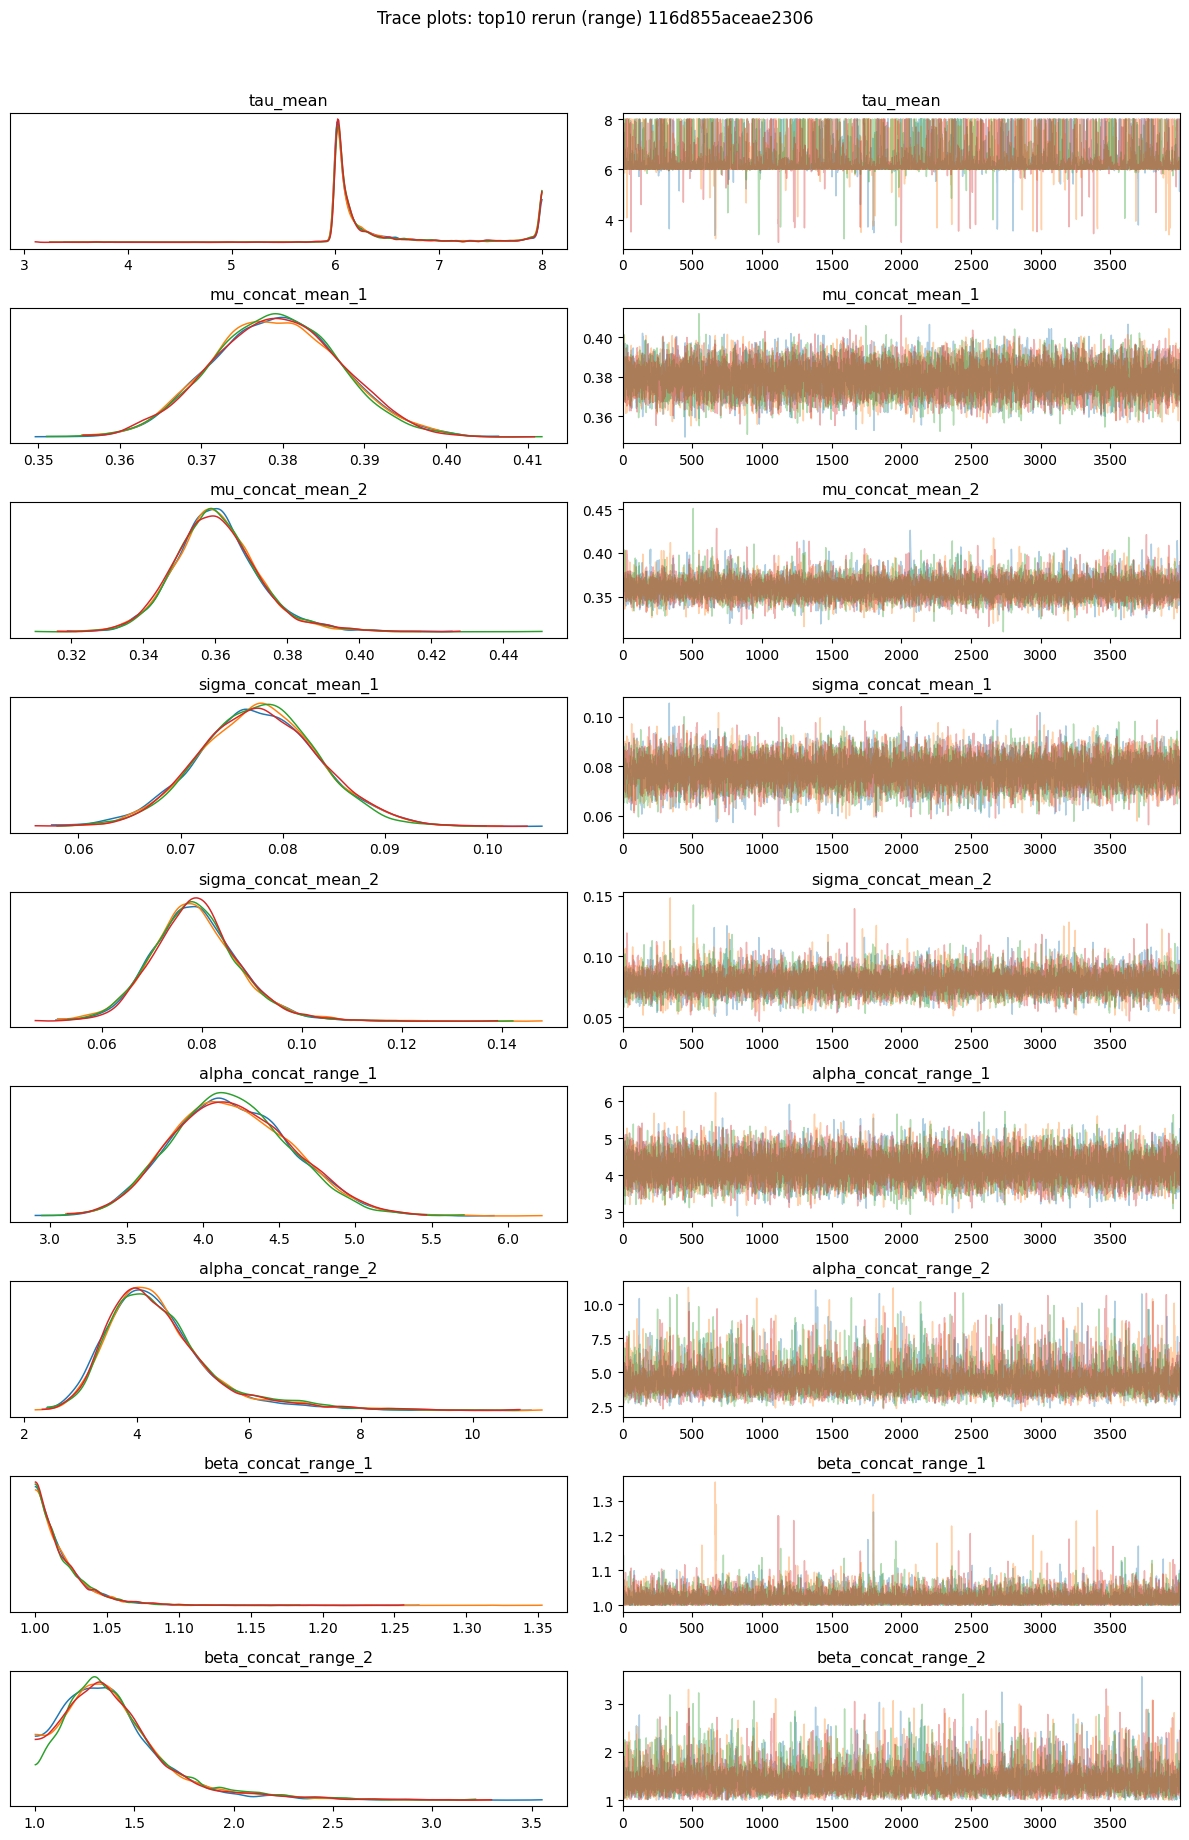
\includegraphics[width=\textwidth]{trace.png}
		\caption{Визуализация трассировки MCMC семплирования.}
		\label{fig:trace} % Метка для ссылки
	\end{figure}
	
	\begin{figure}[H]
		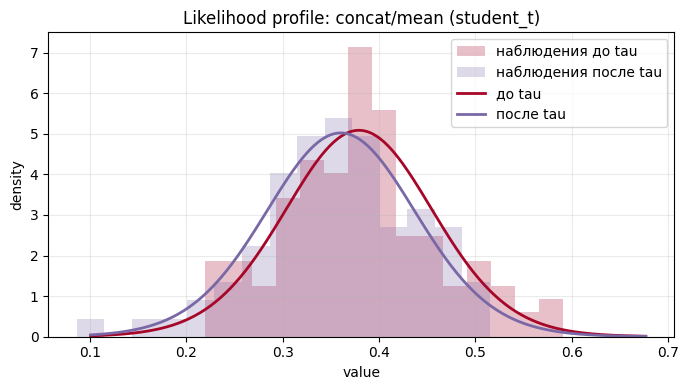
\includegraphics[width=\textwidth]{dist_mean.png}
		\caption{Визуализация апостериорного правдоподобия суточного среднего с гистограммами наблюдений, разделенных точкой разладки.}
		\label{fig:dist_mean} % Метка для ссылки
	\end{figure}
	
	\begin{figure}[H]
		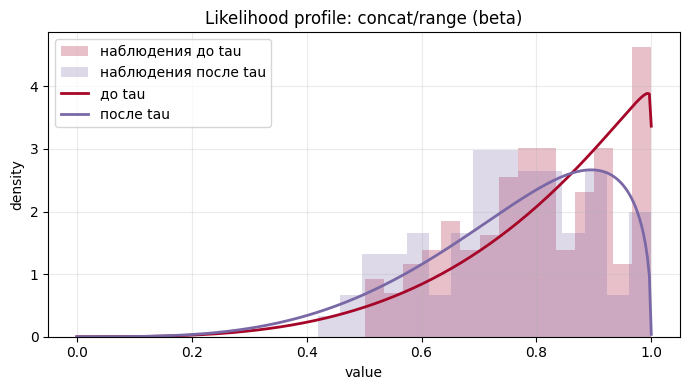
\includegraphics[width=\textwidth]{dist_range.png}
		\caption{Визуализация апостериорного правдоподобия суточного размаха с гистограммами наблюдений, разделенных точкой разладки..}
		\label{fig:dist_range} % Метка для ссылки
	\end{figure}
	
	\begin{figure}[H]
		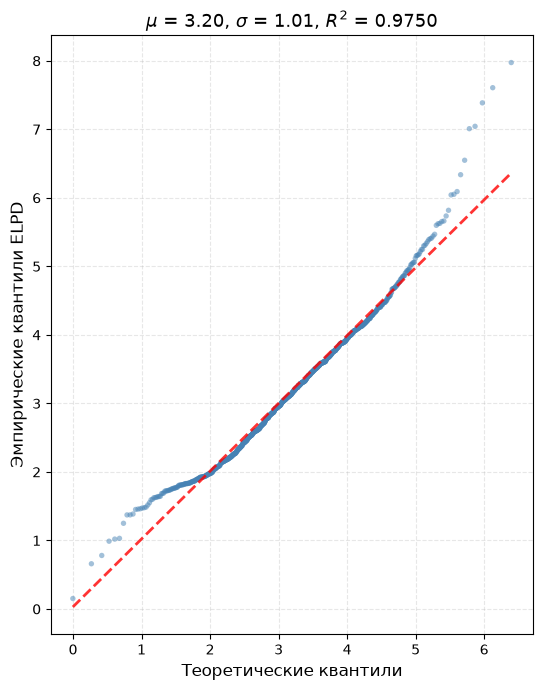
\includegraphics[width=\textwidth]{qq_elpd.png}
		\caption{Q-Q график сравнения распределения ELPD пространства моделей с нормальным законом.}
		\label{fig:qq_elpd} % Метка для ссылки
	\end{figure}
	
	\begin{figure}[H]
		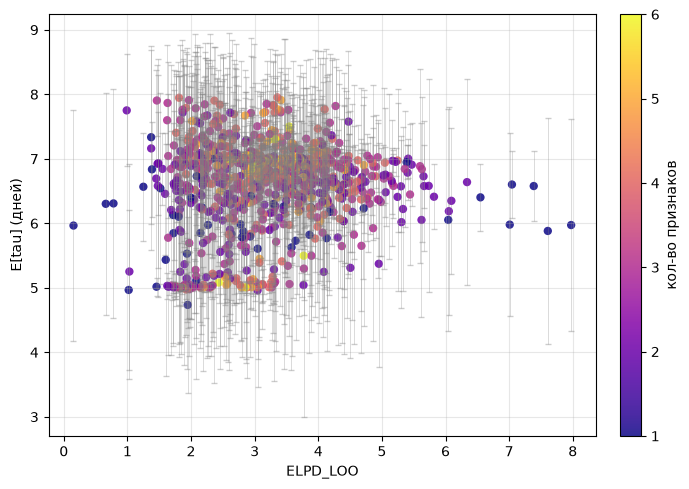
\includegraphics[width=\textwidth]{e_tau.png}
		\caption{График  $\mathbb{E}[\tau]$ по всем моделям. Усы - $\pm std(\tau) $, цвет точки указывает на количество используемых моделью признаков.}
		\label{fig:e_tau} % Метка для ссылки
	\end{figure}
	
	\begin{figure}[H]
		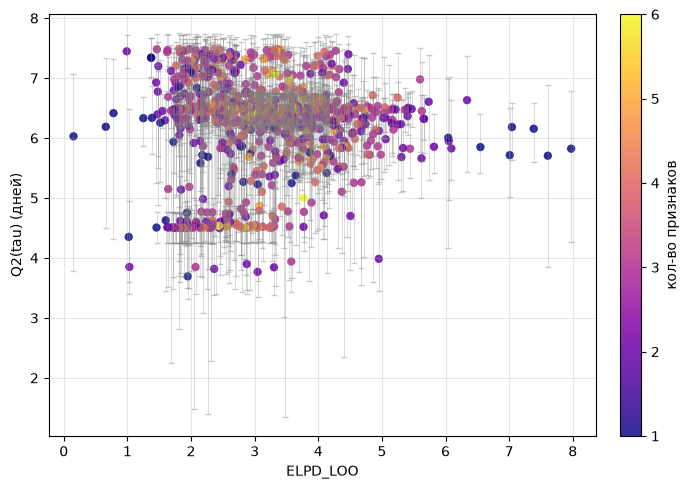
\includegraphics[width=\textwidth]{q2_tau.png}
		\caption{График  $\mathbf{Q}_2(\tau)$ по всем моделям. Усы - $\mathbf{Q}_1(\tau)$ и $\mathbf{Q}_3(\tau)$, цвет точки указывает на количество используемых моделью признаков.}
		\label{fig:q2_tau} % Метка для ссылки
	\end{figure}
	
	
	\begin{lstlisting}[language=Python, caption={Полная реализация \texttt{\_build\_prior}}, label=app-lst:bayes-model]
def run_variant(
title: str,
*,
n_chunks: int,
feature_selection,
parameter_selection: dict | None = None,
rem_profile_params: dict | None = None,
draws: int = 4000,
tune: int = 2000,
nuts_backend: str = "pymc",
chains: int = 4,
cores: int | None = None,
tau_mode: str = "discrete",
tau_lower: int = 2,
tau_upper: int | None = None,
data_norm: np.ndarray | None = None,
plot_likelihood_profiles: bool = True,
likelihood_profile_grid_size: int = 300,
likelihood_profile_log_density_y: bool | set[tuple[str, str]] |
 None = None,
return_likelihood_profiles: bool = False,
):
"""Full scenario run: features -> model -> MCMC -> summary -> 
plots."""
normalized_rem_profile_params: dict[str, int] | None = None
if rem_profile_params is not None:
required_keys = {"window_size_hours", "step_size_hours", 
	"rem_stage"}
missing = sorted(required_keys - set(rem_profile_params))
if missing:
raise ValueError(
"rem_profile_params is missing required keys: "
f"{missing}. Expected keys: {sorted(required_keys)}"
)
w, s, r = _normalize_rem_profile_params(
window_size_hours=rem_profile_params["window_size_hours"],
step_size_hours=rem_profile_params["step_size_hours"],
rem_stage=rem_profile_params["rem_stage"],
)
normalized_rem_profile_params = {
	"window_size_hours": w,
	"step_size_hours": s,
	"rem_stage": r,
}

backend = str(nuts_backend).strip().lower()
if backend in {"numpyro", "blackjax"} and str(tau_mode)
.strip().lower() == "discrete":
print(
"JAX NUTS backend with discrete tau is unsupported; 
using tau_mode='marginalized'."
)
tau_mode = "marginalized"

data_for_run = data_norm if data_norm is not None else
 _RUNTIME_DATA_NORM
if normalized_rem_profile_params is not None and 
data_norm is None:
if _RUNTIME_LAST_EXPORT_CFG is None:
print(
"rem_profile_params were provided, but no prior export
 config is available. "
"Using existing runtime data without recalculation."
)
else:
export_cfg = dict(_RUNTIME_LAST_EXPORT_CFG)
export_cfg.update(normalized_rem_profile_params)
print("Recalculating REM profiles with updated 
rem_profile_params...")
export_result = export_rem_profiles_10days_cached_only(**export_cfg)

prep_cfg = _RUNTIME_LAST_PREPARE_CFG or {}
prep_csv_path = export_result["paths"]["nanpad_output_csv"]
prep_bad_indices = prep_cfg.get("bad_sample_indices", None)
prep = prepare_model_data(
csv_path=prep_csv_path,
bad_sample_indices=prep_bad_indices,
)
set_runtime_data_norm(prep["data_norm"])
data_for_run = prep["data_norm"]
print(
"Recalculation complete: "
f"data_norm shape={data_for_run.shape}, 
csv_path={prep_csv_path!r}"
)

if data_for_run is None:
raise ValueError("data_norm is not set. 
Pass data_norm=... or call set_runtime_data_norm(...).")

print("=" * 90)
print(f"Сценарий: {title}")
print(f"  n_chunks={n_chunks}")
print(f"  feature_selection={feature_selection!r}")
if parameter_selection is not None:
print(f"  parameter_selection={parameter_selection!r}")
if normalized_rem_profile_params is not None:
print(f"  rem_profile_params={normalized_rem_profile_params!r}")
print(
"  note: rem_profile_params trigger recalculation only
 when runtime export "
"and prepare configs are available (or when data_norm is 
passed explicitly)."
)
print(f"  nuts_backend={nuts_backend!r}")
print(f"  tau_mode={tau_mode!r}")
print("=" * 90)

group_data = build_group_data(
data_for_run,
n_chunks=n_chunks,
feature_selection=feature_selection,
)
for group_name, features in group_data.items():
for feat_name, df in features.items():
print(f"Группа '{group_name}', признак '{feat_name}': 
форма {df.shape}")
print(f"Первые 2 строки ({feat_name}):")
print(df.head(2).to_string(index=False))
print()

model = build_changepoint_model(
group_data,
tau_lower=tau_lower,
tau_upper=tau_upper,
parameter_selection=parameter_selection,
tau_mode=tau_mode,
)
trace = sample_model(
model,
draws=draws,
tune=tune,
nuts_backend=nuts_backend,
chains=chains,
cores=cores,
)
available_vars = _available_varnames(trace)
trace_vars = []
summary_vars = []
if "tau" in available_vars:
trace_vars.append("tau")
summary_vars.append("tau")
if "tau_mean" in available_vars:
trace_vars.append("tau_mean")
summary_vars.append("tau_mean")

for group_name, features in group_data.items():
for feat_name in features.keys():
for param_name in ("mu", "sigma", "alpha", "beta"):
p1 = f"{param_name}_{group_name}_{feat_name}_1"
p2 = f"{param_name}_{group_name}_{feat_name}_2"
if p1 in available_vars and p2 in available_vars:
trace_vars.extend([p1, p2])
summary_vars.extend([p1, p2])
nu_name = f"nu_{group_name}_{feat_name}"
if nu_name in available_vars:
summary_vars.append(nu_name)

if summary_vars:
summary = summary_from_trace(trace, summary_vars)
print(summary[["mean", "sd", "r_hat", "ess_bulk", 
"ess_tail"]].to_string())
else:
summary = pd.DataFrame()
print("Summary: no scalar parameters selected for 
compact table.")

diverging = _sampler_stat(trace, "diverging")
n_div = int(np.asarray(diverging).sum())
print(f"Дивергенции: {n_div}")

energy = np.asarray(_sampler_stat(trace, "energy"),
 dtype=float).reshape(-1)
if energy.size > 1 and np.var(energy) > 0:
bfmi = float(np.mean(np.diff(energy) ** 2) / np.var(energy))
print(f"BFMI (approx): {bfmi:.3f}")
else:
print("BFMI (approx): недостаточно данных.")

support, probs = tau_probabilities(trace)
print("Вероятности tau:")
for k, p in zip(support, probs):
print(f"  P(tau={k}) = {p:.3f}")
map_idx = int(np.argmax(probs))
print(f"MAP tau: {int(support[map_idx])}, концентрация:
 {float(probs[map_idx]):.3f}")

plot_trace_and_tau(trace, trace_vars, title_prefix=title)
plot_posteriors_like_script(trace, group_data=group_data, 
title_prefix=title)
likelihood_profiles = feature_likelihood_profiles(
trace,
group_data=group_data,
parameter_selection=parameter_selection,
grid_size=likelihood_profile_grid_size,
plot=plot_likelihood_profiles,
log_density_y=likelihood_profile_log_density_y,
)
if return_likelihood_profiles:
return trace, summary, likelihood_profiles
return trace, summary
		
	\end{lstlisting}
	
	
\end{document}
